\documentclass[tikz,border=2mm]{standalone}

\usetikzlibrary{babel, positioning, shapes.multipart}
 \tikzset{
state/.style={
       rectangle split,
       rectangle split parts=5,
       rectangle split part fill={pink,red!30,red!30,blue!20,blue!20},
       rounded corners,
       draw=black, very thick,
       minimum height=2em,
       text width=3cm,
       inner sep=2pt,
       text centered,
       }
}
\usetikzlibrary{matrix,fit}

\begin{document}

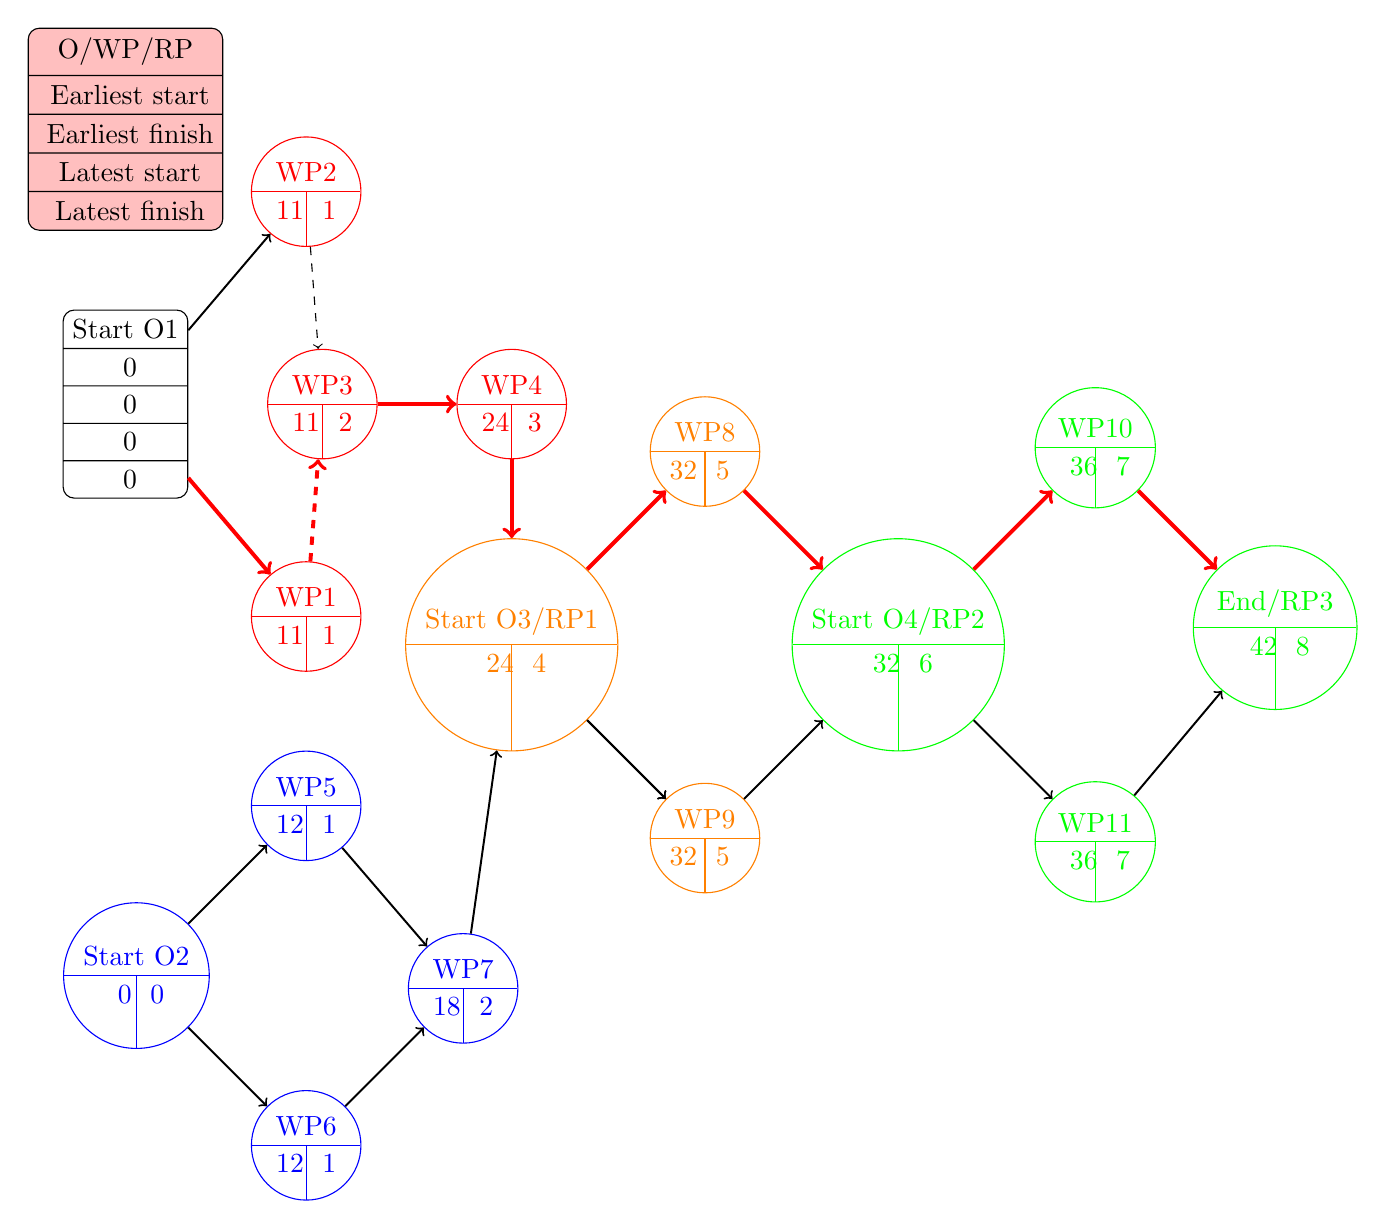
\begin{tikzpicture}[
    circle/.style={
            circle split,
            draw,
            path picture={\draw (path picture bounding box.center)--(path picture bounding box.south);}}]

%O1====================================================================          
\node[rectangle split,rectangle split parts=5,draw,text centered,rounded corners] (1) {Start O1 \nodepart{two} \ 0 \nodepart{three} \ 0  \nodepart{four} \ 0  \nodepart{five} \ 0};
\node[circle,color=red, below right=of 1] (2) {WP1\nodepart{lower} 11\ \ 1};
\node[circle,color=red, above right=of 1] (3) {WP2\nodepart{lower} 11\ \ 1};
\node[circle,color=red, right=of 1] (4) {WP3\nodepart{lower} 11\ \ 2};
\node[circle,color=red, right=of 4] (5) {WP4\nodepart{lower} 24\ \ 3};

\node[rectangle split,rectangle split parts=5,draw,text centered,rounded corners,fill=pink,above=of 1] (0) {O/WP/RP \nodepart{two} \ Earliest start \nodepart{three} \ Earliest finish  \nodepart{four} \ Latest start  \nodepart{five} \ Latest finish};

%\node[circle,fill=pink,above=of 1] (0) {O/WP/RP\nodepart{lower} Time\ \ Slack};

\draw[->,red,line width=0.5mm] (1)--(2) node[midway, right]{};
\draw[->,line width=0.25mm] (1)--(3) node[midway, right]{};
%\draw[->,dashed] (2)--(3);
\draw[->,red,line width=0.5mm,dashed] (2)--(4) node[midway, right]{};
\draw[->,dashed] (3)--(4) node[midway, right]{};
\draw[->,red,line width=0.5mm] (4)--(5) node[midway]{};
%=======================================================================

%O2====================================================================          
\node[circle,color=blue, below=of 2] (7) {WP5\nodepart{lower} 12\ \ 1};
\node[circle,color=blue,below left=of 7] (6) {Start O2\nodepart{lower}\ 0\  \ 0};


\node[circle,color=blue, below right=of 6] (8) {WP6\nodepart{lower} 12\ \ 1};
\node[circle,color=blue, above right=of 8] (9) {WP7\nodepart{lower} 18\ \ 2};

%\node[circle, right=of 4] (5) {WP4\nodepart{lower} 99\ \ 99};


\draw[->,line width=0.25mm] (6)--(7) node[midway, right]{};
\draw[->,line width=0.25mm] (6)--(8) node[midway, right]{};
%\draw[->,dashed] (2)--(3);
\draw[->,line width=0.25mm] (7)--(9) node[midway, right]{};
\draw[->,line width=0.25mm] (8)--(9) node[midway, right]{};
%\draw[->] (4)--(5) node[midway]{t(5)};
%=======================================================================

%O3====================================================================          
\node[circle,color=orange,below=of 5] (10) {Start O3/RP1\nodepart{lower}\ 24 \ 4};
\node[circle,color=orange,above right=of 10] (11) {WP8\nodepart{lower}\  \hspace{-0.1 in}32\  \ 5};
\node[circle,color=orange,below right=of 10] (12) {WP9\nodepart{lower}\  \hspace{-0.1 in}32\  \ 5};
\draw[->,red,line width=0.5mm] (5)--(10) node[midway, right]{};
\draw[->,line width=0.25mm] (9)--(10) node[midway, right]{};
\draw[->,red,line width=0.5mm] (10)--(11) node[midway, right]{};
\draw[->,line width=0.25mm] (10)--(12) node[midway, right]{};

%O4====================================================================          
\node[circle,color=green,below right=of 11] (13) {Start O4/RP2\nodepart{lower}\ 32\  \ 6};
\node[circle,color=green,above right=of 13] (14) {WP10\nodepart{lower}\  36\  \ 7};
\node[circle,color=green,below right=of 13] (15) {WP11\nodepart{lower}\  36\  \ 7};
\node[circle,color=green,below right=of 14] (16) {End/RP3 \nodepart{lower}\  42\  \ 8};
\draw[->,red,line width=0.5mm] (13)--(14) node[midway, right]{};
\draw[->,line width=0.25mm] (13)--(15) node[midway, right]{};
%\draw[->] (10)--(11) node[midway, right]{};
\draw[->,line width=0.25mm] (10)--(12) node[midway, right]{};
\draw[->,red,line width=0.5mm] (11)--(13) node[midway, right]{};
\draw[->,line width=0.25mm] (12)--(13) node[midway, right]{};
\draw[->,red,line width=0.5mm] (14)--(16) node[midway, right]{};
\draw[->,line width=0.25mm] (15)--(16) node[midway, right]{};







\end{tikzpicture}

\end{document}

% B
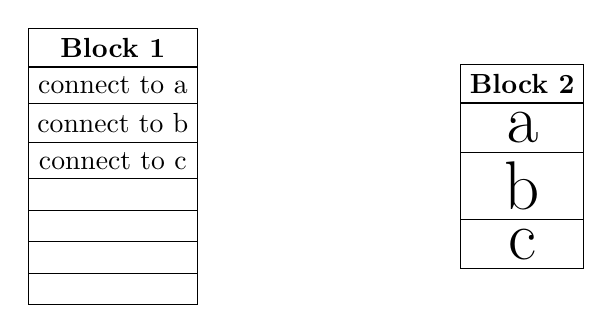
\begin{tikzpicture}[
  grow=right,    
  level 1/.style={sibling distance=3.5cm,level distance=5.2cm},
  edge from parent/.style={draw=white},
]

\node[name=block1, rectangle split, rectangle split parts=8, draw=black]
  { \textbf{Block 1}
    \nodepart{second} connect to a
    \nodepart{third} connect to b
    \nodepart{fourth} connect to c
  }
  child {
    node[name=block2, rectangle split, rectangle split parts=4, draw=black]
     {  \textbf{Block 2}
        \nodepart{second} \Huge{a}
        \nodepart{third} \Huge{b}
        \nodepart{fourth} \Huge{c}
    }
};
\end{tikzpicture}


%C
\tikzset{
    table nodes/.style={
        rectangle,
        draw=black,
        align=center,
        minimum height=7mm,
        text depth=0.5ex,
        text height=2ex,
        inner xsep=0pt,
        outer sep=0pt
    },      
    table/.style={
        matrix of nodes,
        row sep=-\pgflinewidth,
        column sep=-\pgflinewidth,
        nodes={
            table nodes
        },
        execute at empty cell={\node[draw=none]{};}
    }
}
\begin{tikzpicture}

\matrix (first) [table,text width=7mm,name=table]
{
A   & B & C & D\\
E   &   &   & F\\
};
\node[draw,fit=(table-2-2)(table-2-3),table nodes]{F};


\matrix (first) [table,text width=7mm,name=table]
{
A   & B & C & D\\
E   &   &   & F\\
};
\node[draw,fit=(table-2-2)(table-2-3),table nodes]{F};

\end{tikzpicture}

